\chapter{Teori}
\label{cha:theory}

\section{Punktmoln}
På senare år har det blivit möjligt att representera objekt i form av ett 3D-representerat punkt\-moln. Detta har blivit möjligt på grund av utvecklandet av kameror samt laserskannrar. Ett punktmoln är alltså en mängd av punkter i ett tredimensionellt koordinatsystem som representerar ett objekt. Punkterna i punktmolnet representerar ofta de yttre kanterna av objektet \cite{point_cloud}.

Det finns två stycken typer av punktmoln, ett så kallat komplett punktmoln och ett icke komplett punktmoln. Ett komplett punktmoln, se figur \ref{fig:point_cloud_torus}, betyder att punktmolnet innehåller samtliga punkter som behövs för att representera objektet. Ett icke komplett punktmoln, se figur \ref{fig:point_cloud_church}, betyder att punktmolnet inte innehåller tillräckligt med punkter för att representera objektet. 

\begin{figure}[H]
	\centering
	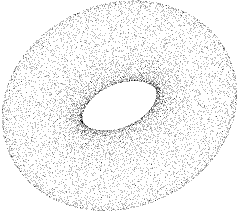
\includegraphics[width=30mm]{figures/Point_cloud_torus1.png}
	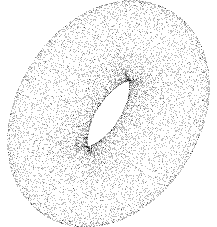
\includegraphics[width=30mm]{figures/Point_cloud_torus2.png}
	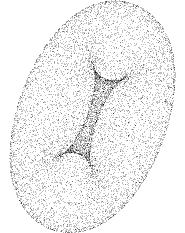
\includegraphics[width=30mm]{figures/Point_cloud_torus3.png}
	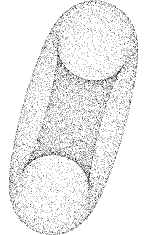
\includegraphics[width=30mm]{figures/Point_cloud_torus4.png}
	\caption{Ett komplett punktmoln som representerar ett torus objekt.}
	\label{fig:point_cloud_torus}
\end{figure}

\begin{figure}[H]
	\centering
	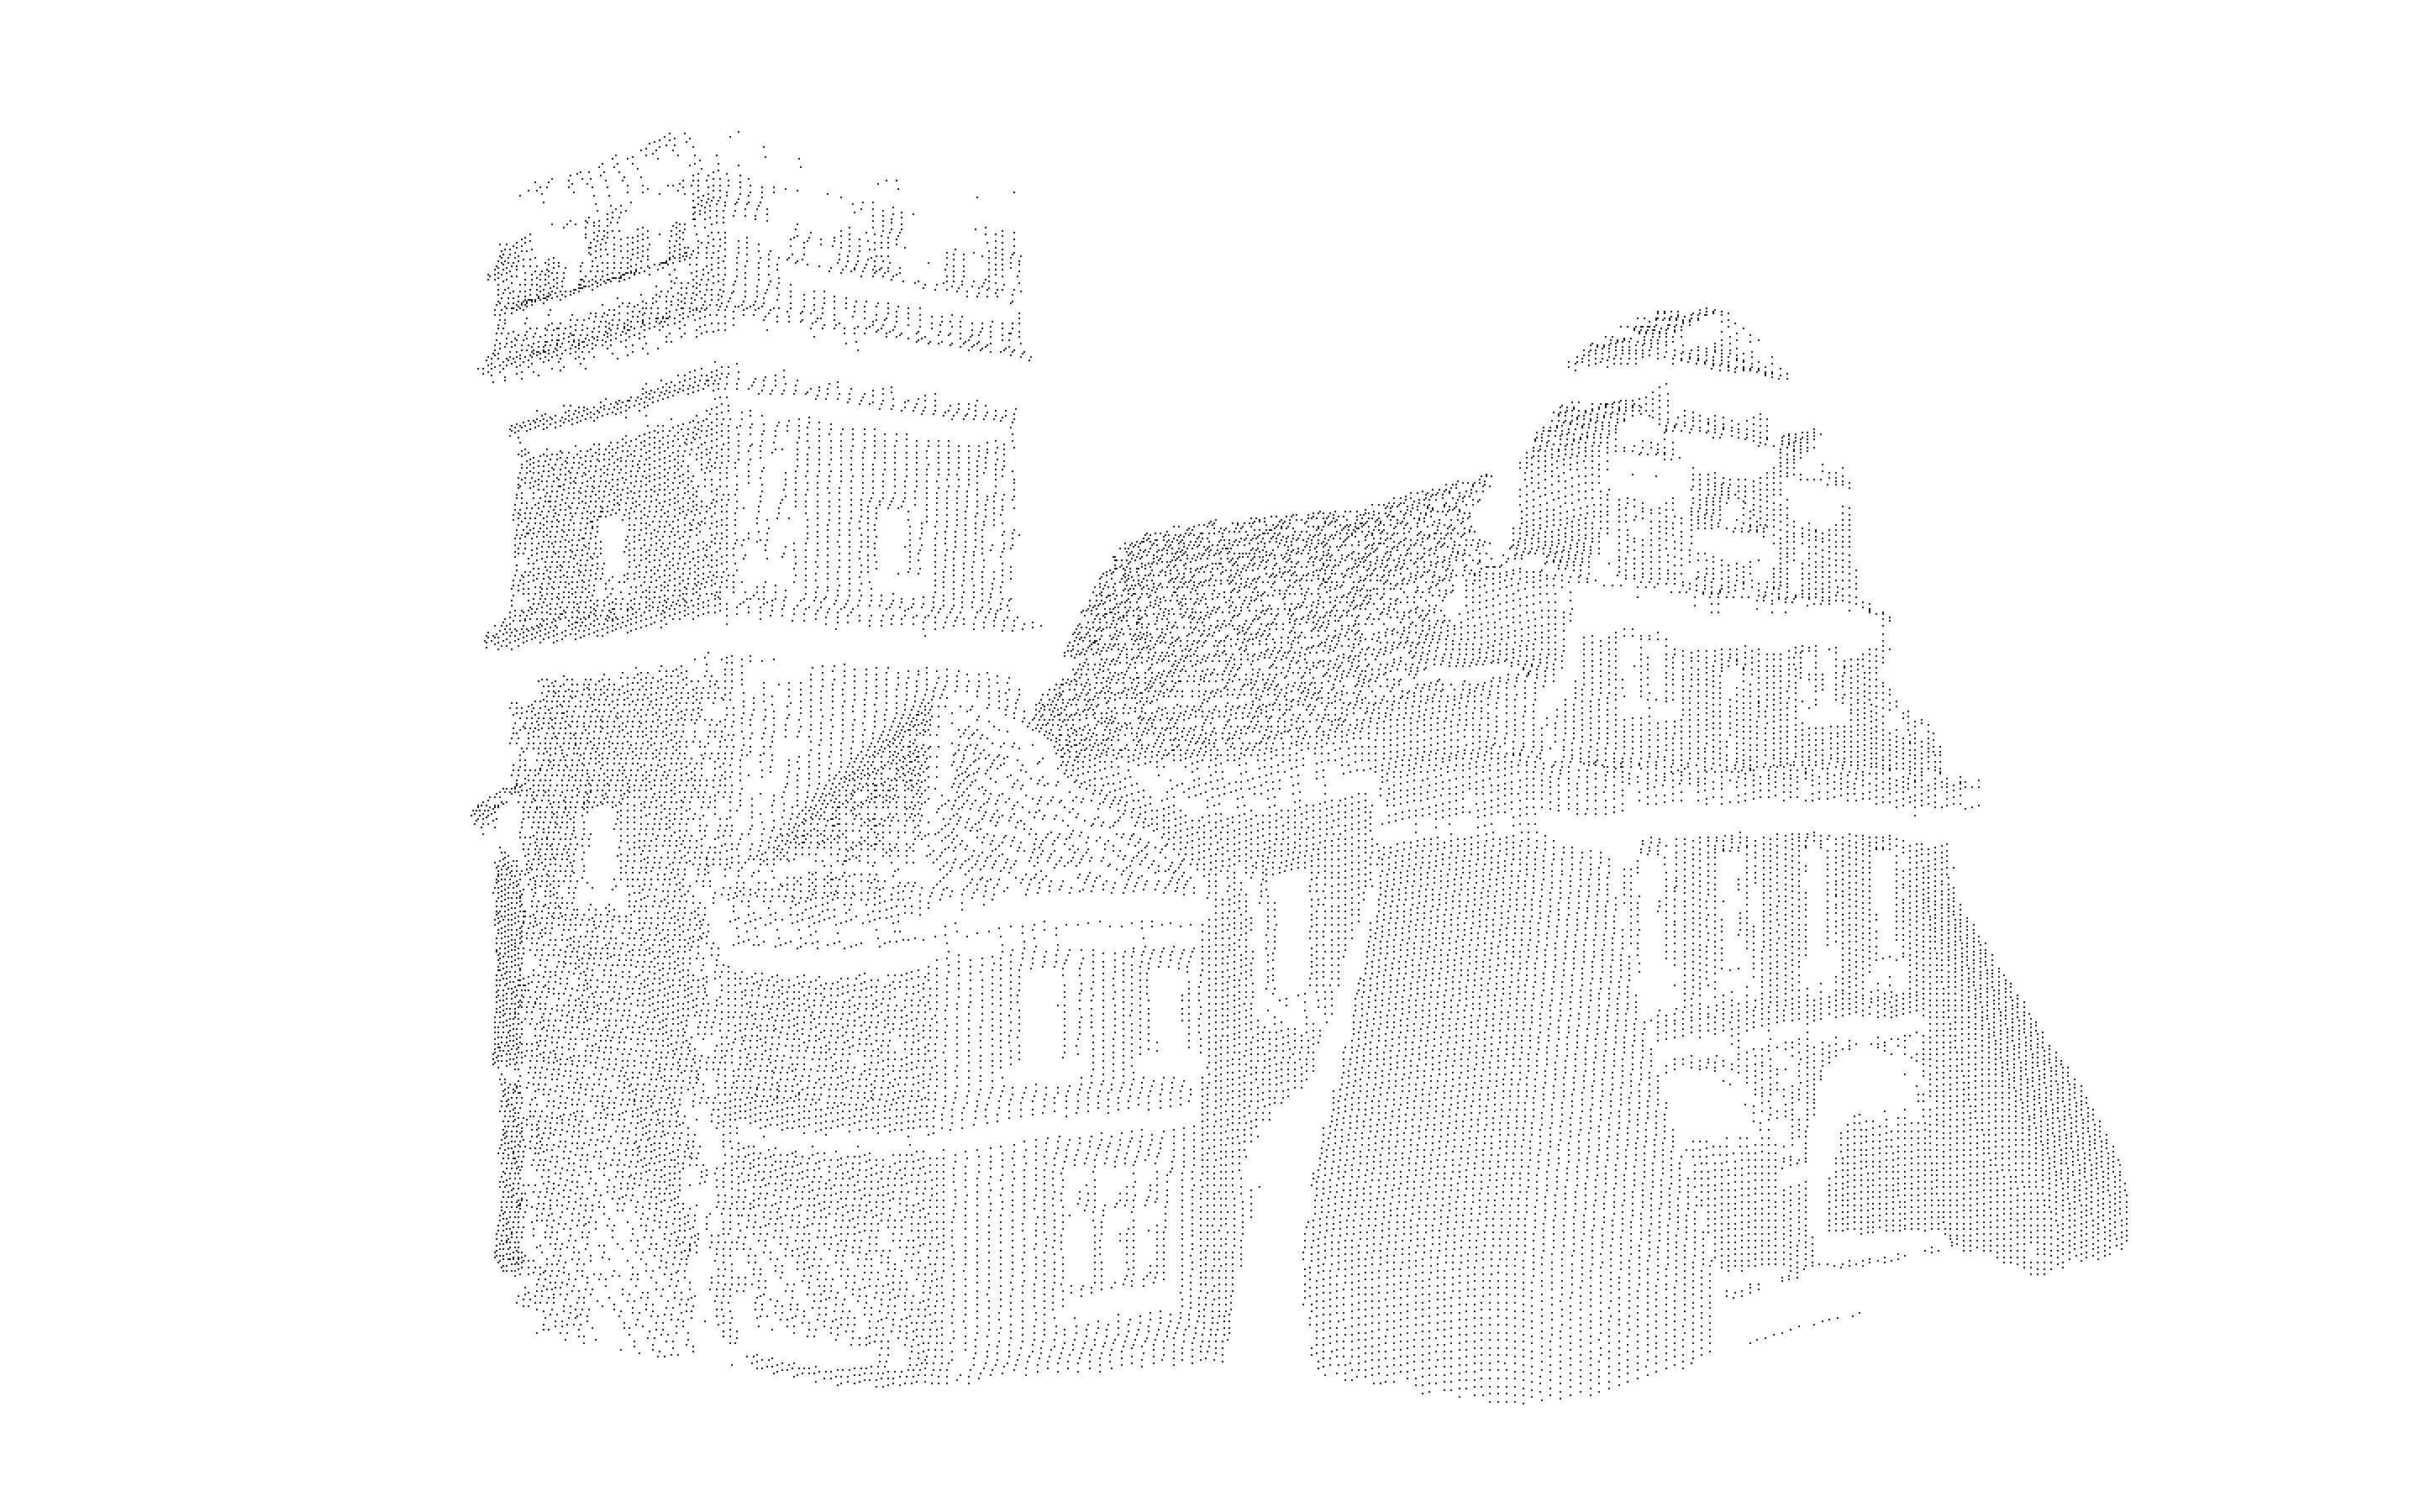
\includegraphics[width=100mm]{figures/icke_komplett_moln_kyrka.png}
	\caption{Ett icke komplett punktmoln som representerar en del av en kyrka.}
	\label{fig:point_cloud_church}
\end{figure}

\section{Point Cloud Library}
Point Cloud Library (PCL) är ett bibliotek till C++. PCL presenterar ett avancerat tillvägagångssätt angående ämnet 3D-uppfattning och är tänkt att ge stöd för vanliga 3D-byggstenar som olika applikationer behöver. Biblioteket innehåller algoritmer för:

\begin{itemize}
	\item filtrering
	\item registrering
	\item segmentering
	\item modellanpassning
	\item ytrekonstruering
	\item funktionsestimering.
\end{itemize}
PCL är alltså ett bibliotek avsett att ge stöd till att behandla punktmolnsdata, i form av olika bearbetningsalgoritmer \cite{rusu20113d}.

Varje algoritm i PCL är definierad via basklasser. Dessa basklasser försöker integrera all vanlig funktionalitet tillsammans med algoritmerna som sedan används igenom hela kedjan i den önskade processen. Detta gör att implementeringen av den aktuella algoritm hålls modulär och tydlig. Den grundläggande kedjan för en önskad process i PCL är som följer:

\begin{itemize}
	\item skapa bearbetningsobjektet (filtrering, registrering, segmentering, etc.)
	\item skicka in det givna punktmolnets data till modulen
	\item ange parametrar
	\item gör beräkningen för att få resultatet.
\end{itemize}

PCL använder sig av sitt egna visualiseringsbibliotek, baserat på visualiseringsverktyget VTK \cite{VTK_book}, för att visualisera punktmoln. PCL visualiseringsbibliotek integrerar PCL med VTK med syftet att snabbt kunna visualisera resultaten av de olika algoritmernas arbete. Nedan beskrivs de olika områderna som PCLs algoritmer behandlar \cite{rusu20113d}.

\subsection{Filtrering}
PCLs filtreringsbibliotek innehåller algoritmer för att filtrera ett punktmoln ifrån skräppunkter. Dessa skräppunkter kan uppstå vid skanning av ett objekt eftersom avståndskameran kan reagera på bakgrunden och inte bara på objektet. Det gör att skräppunkter infaller i punkmolnet. För att kunna behandla punktmolnet måste dessa skräppunkter först filtreras bort.

PCL har stöd för fler olika metoder för filtrering. Första steget är att ta bort alla punkter som ligger utanför ett visst intervall av koordinater för att ta bort sådant som måste ligga utanför det skannade objektet. I nästa steg kontrolleras det för varje punkt hur många grannar den punkten har inom en viss radie. Alla punkter som har under ett visst antal grannar tas bort vilket leder till att enstaka punkter som inte ligger i närheten av något objekt tas bort \cite{pcl_filtering}.

För att undvika att punktmoln blir för stora, det vill säga får för många punkter så att de tar för lång tid att behandla, kan nedsampling användas för att ta bort punkter och samtidigt uppskatta den yta som representeras så nära som möjligt. För att göra detta i PCL delas punktmolnet som ska nedsamplas in i voxels, vilket kan ses som att punktmolnet delas in i ett antal kuber. Sedan ersätts alla punkter i varje kub med en punkt som ligger i centrum för alla punkterna i kuben. På detta sätt ges en nära uppskattning av den representerade ytan med mycket färre punkter än det ursprungliga punktmolnet \cite{voxel_grid}.
 
\subsection{Segmentering}
PCLs segmenteringsbibliotek innehåller algoritmer för att dela in ett punktmoln i olika kluster. Dessa kluster används för att bryta ner molnet i olika beståndsdelar som kan behandlas oberoende av andra delar. Detta görs ofta för att bearbeta olika eller en specifik del av ett punktmoln. Till exempel kan ett plan segmenteras utifrån en uppsättning av punkter om så önskas \cite{pcl_segmentation}. 
 
\subsection{Modellanpassning}
Modellanpassning i PCL innebär att det finns färdiga metoder och modeller, till exempel plan och cylindrar, som kan kombineras och användas för att upptäcka specifika modeller i ett punktmoln. Detta sub-bibliotek används flitigt av segmenteringsbiblioteket för att upptäcka segment av vanliga geometriska figurer \cite{pcl_model_fitting}.

\subsection{Registrering}
Att anpassa olika punkter i ett punktmoln så att de representerar en komplett modell över objektet kallas för att punktmolnsregistrering. Det är ett stort problem inom området och PCL erbjuder ett registreringsbibliotek för ändamålet. Målet med registreringen är alltså hitta de relativa positionerna och orienteringarna för de separata punkmolnen (tagna från olika vyer) så att varje punkt i respektive moln överlappar perfekt med varandra \cite{pcl_registration}. För mer information angående registreringen och dess algoritmer, så behandlas det området i Michaels Karlssons individuella utredning, se avsnitt \ref{cha:indiv-report-karlsson}.

\subsection{Ytrekonstruering}
PCLs ytrekonstrueringsbibliotek innehåller algoritmer för att rekonstruera de ursprungliga ytorna från 3D-skanningar. Beroende på uppgiften kan PCL till exempel rekonstruera en ojämn yta till en jämn, en meshrepresentation av ett komplett punktmoln eller en yta med normaler \cite{pcl_surface_reconstruction}. 

Att rekonstruera en ojämn yta till en jämn kan vara viktigt om molnet är bullrigt, eller om det består av flera skanningar som inte är perfekt anpassade. PCLs ytrekonstrueringsbibliotek kan även skapa en konkav modell av ett punktmoln. Detta kan vara bra om till exempel gränserna i ett punktmoln behöver extraheras \cite{pcl_surface_reconstruction}.

Att mesha ett punktmoln görs efter att punktmolnen har registreras så de bildar ett komplett punktmoln. Att skapa en meshrepresentation av ett komplett punktmoln innebär att skapa en yta utan punkter. Meshrepresentationen av punktmolnet är alltså en vattentät 3D-modell uppbyggd av polygoner. Den algoritm som används för att mesha ett punktmoln i detta projekt är en trianguleringsalgoritm som körs på ett punktmoln med normaler för att erhålla en yta baserad på grannarna till respektive punkt. För detta krävs alltså ett punktmolnsobjekt som innehåller normalerna till varje punkt i punktmolnet. I detta punktmoln med normaler kan sedan önskade parametrar sättas innan själva trianguleringsalgoritm körs för att generera den önskade meshen \cite{pcl_surface_reconstruction}\cite{pcl_triangulation_algorithm}. 

\subsection{Funktionsestimering}
PCLs funktionsbibliotek innehåller datastrukturer och mekanismer för att estimera 3D-funktioner från punktmolnsdata. 3D-funktioner beskriver geometriska mönster vid en viss punkt baserat på informationen som finns tillgänglig kring punkten \cite{pcl_feature_estimation}.

\section{3D-skrivare}
En 3D-skrivare kan användas för att skriva ut 3D-objekt i plast utifrån modeller i en dator. För att kunna göra detta har skrivaren ett styrkort som exekverar så kallad G-code \cite{gcode} vilken säger vilka motorer som ska flyttas och hur mycket. En 3D-modell som är sparad i datorn i form av en mesh måste alltså behandlas genom att använda en algoritm för att generera G-code utifrån modellen. Detta görs ofta genom en typ av programvara som kallas för slicer. Namnet kommer av att programmet delar upp modellen i olika lager och sedan genererar hur skrivaren måste röra för att skriva ut ett lager. På detta sätt byggs sedan hela den ursprungliga modellen upp lager för lager. Två vanliga slicer-programvaror är \textit{Cura} \cite{cura} och \textit{Slic3r} \cite{slic3r}.

\section{Systemanatomi}
En systemanatomi, vars viktigaste egenskap är enkelheten, är en visuell beskrivning av ett system som gör det enkelt för samtliga i utvecklingsgruppen att förstå systemet och dess interna beroenden. Systemanatomin är särskilt användbar vid utveckling av stora komplexa system i agila utvecklingsgrupper eftersom det ger en gemensam syn över systemet. En systemanatomi kan inte ersätta andra modeller eller designverktyg utan det är enbart ett annat sätt att beskriva designen av systemet \cite{system_anatomy}.


\section{Hållbar utveckling}
Hållbar utveckling är en relevant aspekt i dagens utveckling av programvaror eftersom de används kontinuerligt av samhället. Effekterna som en programvara bidrar med i samhället beror på hur den har producerats och hur den används av konsumenterna. Detta gör att effekterna som en programvara bidrar med i samhället kan vara både positiva men också djupt negativa \cite{raturi2014developing}. Hållbarhet definieras som \textit{förmåga att uthärda} och \textit{bevara funktionen hos ett system under en utsträckt tidsperiod}. Att analysera hållbarhet hos ett mjukvarusystem innebär för de som utvecklar systemet att ha dessa fyra områden i åtanke \cite{lago2015framing}:

\begin{itemize}
	\item Ekonomiskt -  Systemet ska bevara kapital och värde.
	\item Socialt - Systemet ska underhålla samhället.
	\item Miljö - Systemet ska skydda mänskliga välfärden genom att skydda naturens tillgångar.
	\item Tekniskt - Systemet ska utvecklas för att stödja långtidsanvändning.
\end{itemize}
En mer ingående beskrivning om hur vårat projekt främjar hållbar utveckling diskuteras i avsnitt \ref{disc:hållbar_utveckling}.


%%%%%%%%%%%%%%%%%%%%%%%%%%%%%%%%%%%%%%%%%%%%%%%%%%%%%%%%%%%%%%%%%%%%%%
%%% theory.tex ends here
